\documentclass[10pt,a4paper,ngerman]{article}
\usepackage[margin=2.5cm]{geometry}
\usepackage[T1]{fontenc}
\usepackage[utf8]{inputenc} % Zeichensatz
\usepackage[ngerman]{babel} % Sprachpaket
\usepackage{amsmath}  % Mathematik
\usepackage{amsfonts} % Mathematik
\usepackage{amssymb}  % Mathematik
\usepackage{palatino} % Schriftart
\usepackage{titling}  % für eigene Überschrift
\usepackage{graphicx}
\usepackage{subcaption}
\usepackage{wasysym}  % enthält Symbole, wie Quadrate (für Multiple Choice Fragen)
\usepackage{dirtree}  % Verzeichnisbäume
\usepackage{hyperref} % Hyperlinks und andere Verlinkungen

% Package für die Kopf- und Fußzeilen
\usepackage{scrlayer-scrpage}
\pagestyle{scrheadings}
\clearpairofpagestyles % Die einzelnen Bereiche leeren

% Quelltext-Listings 
\usepackage{listings} % Listings
\usepackage{color}    % Syntax-Highlighting

% Farben definieren (für Syntax-Highlighting)
\definecolor{middlegray}{rgb}{0.5,0.5,0.5}
\definecolor{lightgray}{rgb}{0.8,0.8,0.8}
\definecolor{darkgray}{gray}{0.2} % gray: nur ein Wert wird angegeben, welcher dem Grauton entspricht
\definecolor{comment}{rgb}{0.0,0.5,0.0}
\definecolor{keywordcolor}{rgb}{0.0, 0.28, 0.67}

\newcommand{\lstfs}{\fontsize{10}{12}}

% Listings formatieren
\lstset{
   	basicstyle=\ttfamily\lstfs,
   	keywordstyle=\bfseries\ttfamily\color{keywordcolor},
   	stringstyle=\color{darkgray}\ttfamily,
   	commentstyle=\color{comment}\ttfamily,
  	emph={square}, 
   	emphstyle=\ttfamily,
   	emph={[2]root,base},
   	emphstyle={[2]\ttfamily},
   	showstringspaces=false,
   	flexiblecolumns=false,
   	tabsize=2,
   	numbers=left,
   	numberstyle=\tiny,
   	numberblanklines=false,
   	stepnumber=5,
   	firstnumber=1,
 	numberfirstline=true,
   	numbersep=10pt,
	xleftmargin=15pt,
	literate={ö}{{\"o}}1
           {ä}{{\"a}}1
           {ü}{{\"u}}1
           {ß}{{\ss}}1
}



% Metainformationen
\title{Evaluation -- Praktikum 2}
\author{Die Lokalisatoren}

\ihead{}
\chead{}
\ohead{}
\ifoot{}
\cfoot{\pagemark}
\ofoot{}


\newcommand{\doctitle}[1]{\begin{center}\begin{huge}#1\end{huge}\end{center}}

% 1. Variante des docheader (ohne Parameter)
% dann wird der Autor unter der Überschrift ausgegeben
\newcommand{\docheader}{\doctitle{\thetitle}\begin{center}\theauthor\end{center}\hrule\vspace{1em}}

% 2. Variante des docheader (mit Parameter)
% was im Parameter steht wird unter der Überschrift ausgeben
\newcommand{\docheaderparam}[1]{\doctitle{\thetitle}\begin{center}#1\end{center}\hrule\vspace{1em}}

\newcommand{\timbox}[1]{\begin{center}\fbox{\begin{minipage}[t]{0.8\textwidth}#1\end{minipage}}\end{center}}

\newcommand{\code}[1]{\texttt{#1}}

% Für Multiple Choice
\newcommand{\choice}{\item[\Square]}
\newcommand{\cchoice}{\item[\CheckedBox]} % cc = correc choice

\setlength{\parskip}{0em}
\setlength{\parindent}{0em}
\renewcommand{\baselinestretch}{1.5}

\begin{document}

\begin{figure}[t]
	\flushright
	
\includegraphics[width=5cm]{hs-bo-logo}
\end{figure}

\docheader

\section{Wie und wo wir messen}

Auf jede Route werden drei verschiedene Verfahren angewandt: 
\begin{itemize}
	\item FusedLocationProvider - \code{PRIORITY\_HIGH\_ACCURACY} (nachfolgend "`FLP\_HIGH"' genannt)
	\item FusedLocationProvider - \code{PRIORITY\_LOW\_POWER} (nachfolgend "`FLP\_LOW"' genannt)
	\item LocationManager - \code{GPS\_PROVIDER} (nachfolgend "`LM\_GPS"' genannt)
\end{itemize}

Dabei entschieden wir uns für FLP\_HIGH, um die genaueste Positionierung zu erhalten. FLP\_LOW verzichte größtenteils auf GPS- und Wi-Fi-Signale und ermittle die Position über Cell Tower (laut Google). LM\_GPS wurde von uns ausgewählt, um die Genauigkeit von GPS zu der höchstmöglichen Genauigkeit und "`Cell Tower-Genauigkeit"' einzuschätzen bzgl. in Relation zu setzen. \\

Zur Überprüfung der einzelnen Verfahren wurden zwei Routen definiert (Abbildung \ref{fig:routen}). Das Abgehen einer Route folgt dabei folgendem Schema: An Position des ersten Flags wird der "`Start"'-Button betätigt. Sobald die erste Positionierung erfolgte, wird der "`Timestamp"'-Button betätigt und die Route im Schritttempo abgegangen. Jetzt wird der "`Timestamp"'-Button immer betätigt, wenn ein Flag der "`Groundtruth"' passiert wird. Am Ende der Route wird abschließend der "`Timestamp"'- und "`Stop"'-Button betätigt.

\begin{figure}[h!]
	\centering
	\begin{subfigure}[b]{.64\textwidth}
		\centering
        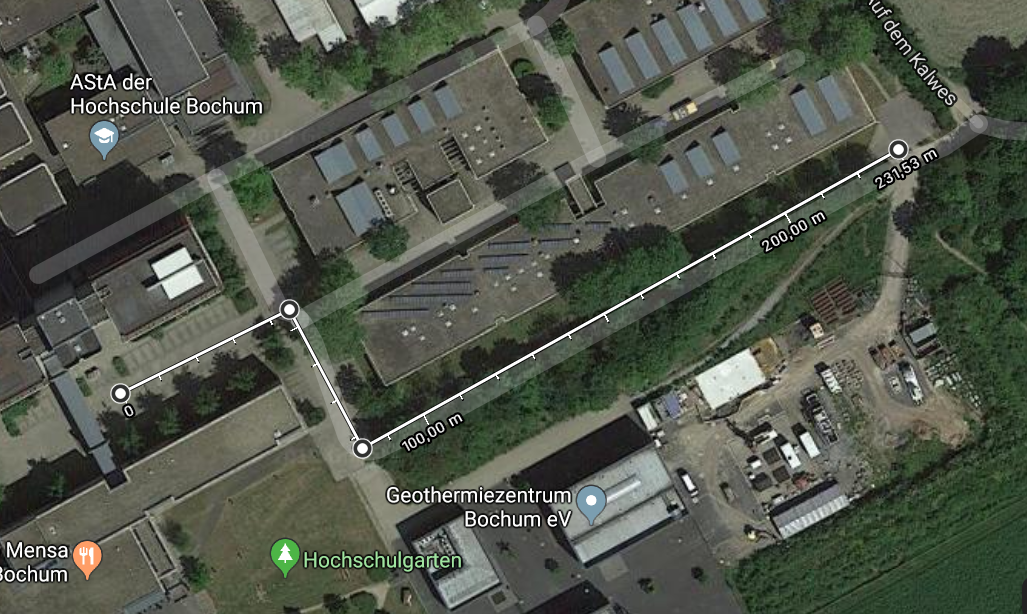
\includegraphics[height=5.2cm]{route1}
        \caption{Route  1 (Outdoors)}
        \label{fig:route1}
    \end{subfigure}
    \begin{subfigure}[b]{.35\textwidth}
    	\centering
        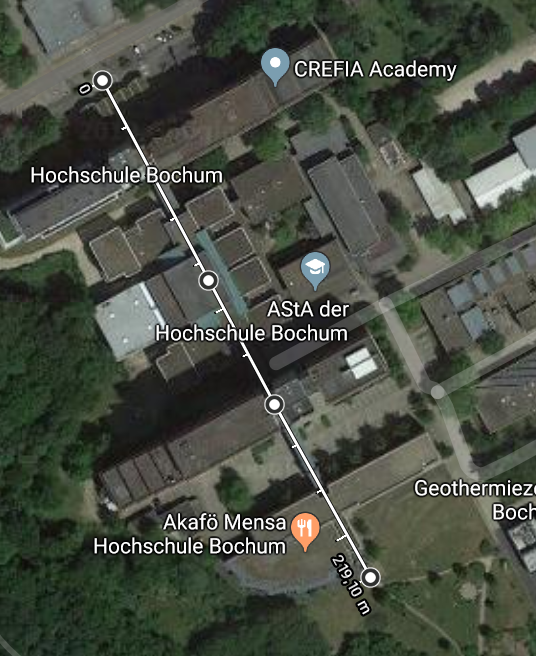
\includegraphics[height=5.2cm]{route2}
        \caption{Route 2 - (Indoors)}
        \label{fig:route2}
    \end{subfigure}
    \caption{Die "`Groundtrouth"' der Routen mit den einzelnen Flags}
    \label{fig:routen}
\end{figure}

\section{Erwartungen}

Wir erwarten, dass die Ergebnisse von FLP\_HIGH genauer sind als die Ergebnisse der übrigen, verwendeten Verfahren. LM\_GPS sollte ähnliche Fehler wie FLP\_LOW ergeben. 

\subsection{Outdoors}

Unserer Erwartung nach sollte FLP\_HIGH die genauesten Werte liefern. Die Fehler von LM\_GPS sollten etwas größer ausfallen, aber dennoch ähnlich aussehen, da FLP\_HIGH größtenteils auf GPS-Daten zurückgreift. \\

FLP\_LOW sollte sehr ungenaue Daten liefern, denn dieser verwendet hauptsächlich Mobilfunksignale zur Positionsbestimmung.

\subsection{Indoors}

Indoors sollten die Positionen, welche rein durch GPS (LM\_GPS) ermittelt wurden, so ungenau sein, dass diese substanzlos sind. \\

Auch die Verfahren des Fused Location Providers sollten Indoors an Genauigkeit verlieren. Zumindest dann, wenn diese sich überwiegend an GPS- bzw. Mobilfunksignalen orientieren. Sollten diese Verfahren auf WiFi-Positionierung umschalten (oder diese dazuschalten), wenn die primär verwendeten Methoden unzureichend sind, könnte auch Indoors eine recht hohe Genauigkeit zustande kommen. Allerdings ist dies reine Spekulation über die interne Logik des Fused Location Providers.

\section{Auswertung}	

Die Verfahren FLP\_HIGH und FLP\_LOW liefern recht ähnliche Daten bzgl. des Fehlers. LM\_GPS ist in beiden Fällen (Indoors und Outdoors) ungenauer als die gewählten Methoden des Fused Location Providers.\\

\textit{Anmerkung}: Die nachfolgenden Daten wurden mit einem Samsung Galaxy S8 erhoben.

\subsection{Technische Umsetzung}

In einem idealen System unter idealen Bedingungen erhält unsere App alle drei Sekunden eine Position vom Betriebssystem -- wie gewünscht. Dann kann zwischen den Punkten der Groundtrouth linear interpoliert werden, um die Genauigkeit zu ermitteln. Der Fehler ergibt sich durch die Distanz der gemessenen Position zur entsprechenden, interpolierten Position der Groundtrouth. \\

Tatsächlich kommt es jedoch durch diverse Umstände dazu, dass die App nicht genau alle drei Sekunden eine Position aus dem Betriebssystem erhält. Meist entstehen Datenreihen, die entweder zu groß oder zu klein sind. Daher müssen die erhobenen Daten zunächst bereinigt werden: Sind die Datenreihen zu groß, so werden die "`überflüssigen"' Positionen gelöscht. Zusätzlich kann es vorkommen, dass die Positionen zu dicht beieinander liegen (zeitlich). Auch diese Daten werden aussortiert. Die Bereinigung der Daten findet ausschließlich im Modus "`Clean Data"' statt. \\

Darüber hinaus kann der Fall eintreten, dass die Listen der gemessenen Daten kürzer sind als die der interpolierten Werte. Dann müsste der Mechanismus zur Datenauswertung in einen anderen Modus schalten. Um die tatsächliche Genauigkeit zu bestimmen -- in diesem Fall -- müssten die interpolierten Positionen mit den gemessenen Positionen gematcht werden (z.B. über Timestamps), anstatt über die Listen parallel zu iterieren.

\subsection{Outdoors}

Die Methoden des Fused Location Providers liefern ähnliche Fehler. Allerdings -- und entgegen der Erwartungen -- sind die Daten von FLP\_LOW genauer als die von FLP\_HIGH. Der Median liegt bei letzterem niedriger, jedoch sind arithmetisches Mittel sowie das 95te Perzentil (Konfidenzlevel 95\%) bei FLP\_LOW deutlich niedriger. Somit ist die Verteilung der Messfehler von FLP\_HIGH rechtsschief. Folglich gibt es nach oben stärkere Abweichungen als bei FLP\_LOW. \\

Die reinen GPS-Werte sind in diesem Versuch deutlich schlechter ausgefallen als erwartet. Der Vermutung nach hätten die Fehler von FLP\_LOW so aussehen sollen, da die Positionierung über das Mobilfunknetz in der Regel (sehr) ungenau ist. Eine Mögliche Erklärung für die ungenauen GPS-Positionen, könnte sein, dass der Startpunkt der Outdoor-Route in einem sogenannten "`Urban Canyon "' liegt. Die Fehlerquelle kann aber auch bei einem fehlerbehafteten Timestamp o.ä. liegen, denn Fehler von 50 Metern sind auf der Karte (Abbildung \ref{fig:map}) nicht zu erkennen.

\renewcommand{\arraystretch}{1.2}
\begin{table}[h!]
	\centering
	\caption{Ergebnisse Route 1 -- Outdoors (Abbildung \ref{fig:route1})}
	\begin{tabular}{|l|l|l|l|}
	\hline
	Fehler (in Meter) & FLP\_HIGH & FLP\_LOW & LM\_GPS \\
	\hline
	\multicolumn{4}{|c|}{\textit{Lagemaße}}\\
	\hline
	Median & $7,615$ & $8,957$ & $32,996$ \\
	Konfidenzlevel 95\% & $18,699$ & $11,949$ & $50,564$ \\
	Arithm. Mittel & $10,007$ & $8,791$ & $28,682$ \\
	\hline
	\multicolumn{4}{|c|}{\textit{Streumaße}}\\
	\hline
	Standardabweichung & $4,627$ & $2,16$ & $16,546$ \\
	Quartilsabstand & $6,891$ & $1,734$ & $32,941$ \\
	\hline
	\end{tabular}
\end{table}

\subsection{Indoors}

In Gebäuden büßen alle Positionierungsvarianten an Genauigkeit ein. FLP\_HIGH liefert dabei noch die genauesten Ergebnisse. FLP\_LOW ist in diesem Fall ungenauer als FLP\_HIGH und die Fehler der reinen GPS-Daten liegen noch höher als bei der Route im Freien. FLP\_LOW ist auch hier viel genauer als erwartet. \\

Daneben ist die Streuung der Fehler deutlich größer. Dies zeigen Standardabweichung und Quartilsabstand an.

\begin{table}[h!]
	\centering
	\caption{Ergebnisse Route 2 -- Indoors (Abbildung \ref{fig:route2})}
	\begin{tabular}{|l|l|l|l|}
	\hline
	Fehler (in Meter) & FLP\_HIGH & FLP\_LOW & LM\_GPS \\
	\hline
	\multicolumn{4}{|c|}{\textit{Lagemaße}}\\
	\hline
	Median & $15,962$ & $15,597$ & $85,378$ \\
	Konfidenzlevel 95\% & $23,583$ & $36,193$ & $106,079$ \\
	Arithm. Mittel & $14,911$ & $16,102$ & $62,419$ \\
	\hline
	\multicolumn{4}{|c|}{\textit{Streumaße}}\\
	\hline
	Standardabweichung & $7,292$ & $10,682$ & $43,719$ \\
	Quartilsabstand & $10,573$ & $16,456$ & $79,299$ \\
	\hline
	\end{tabular}
\end{table}

\subsection{Zusammenfassung}

Im Allgemeinen sind die gewählten Verfahren zur Positionierung im Freien genauer als in Gebäuden. Zusätzlich ist die Streuung der Daten (bzw. Fehler) Indoors größer als Outdoors. Dies sind die Ergebnisse, die den Erwartungen entsprechen. \\

Was nicht den Erwartungen entspricht, ist die Genauigkeit von FLP\_LOW. Neben deutlich höheren Fehlern erwarteten wir unter keinen Umständen das FLP\_LOW unter freiem Himmel genauer ist als FLP\_HIGH. FLP\_LOW sollte unseren Erwartungen nach die ungenaueste Methode mit Fehlern im Bereich von 50 - 100 Metern (oder mehr) sein. Bezüglich der reinen GPS-Daten wird ein Messfehler vermutet (zumindest Outdoors).

\newpage
\section{Screenshots}

\begin{figure}[h!]
    \centering
    \begin{subfigure}[b]{0.35\textwidth}
        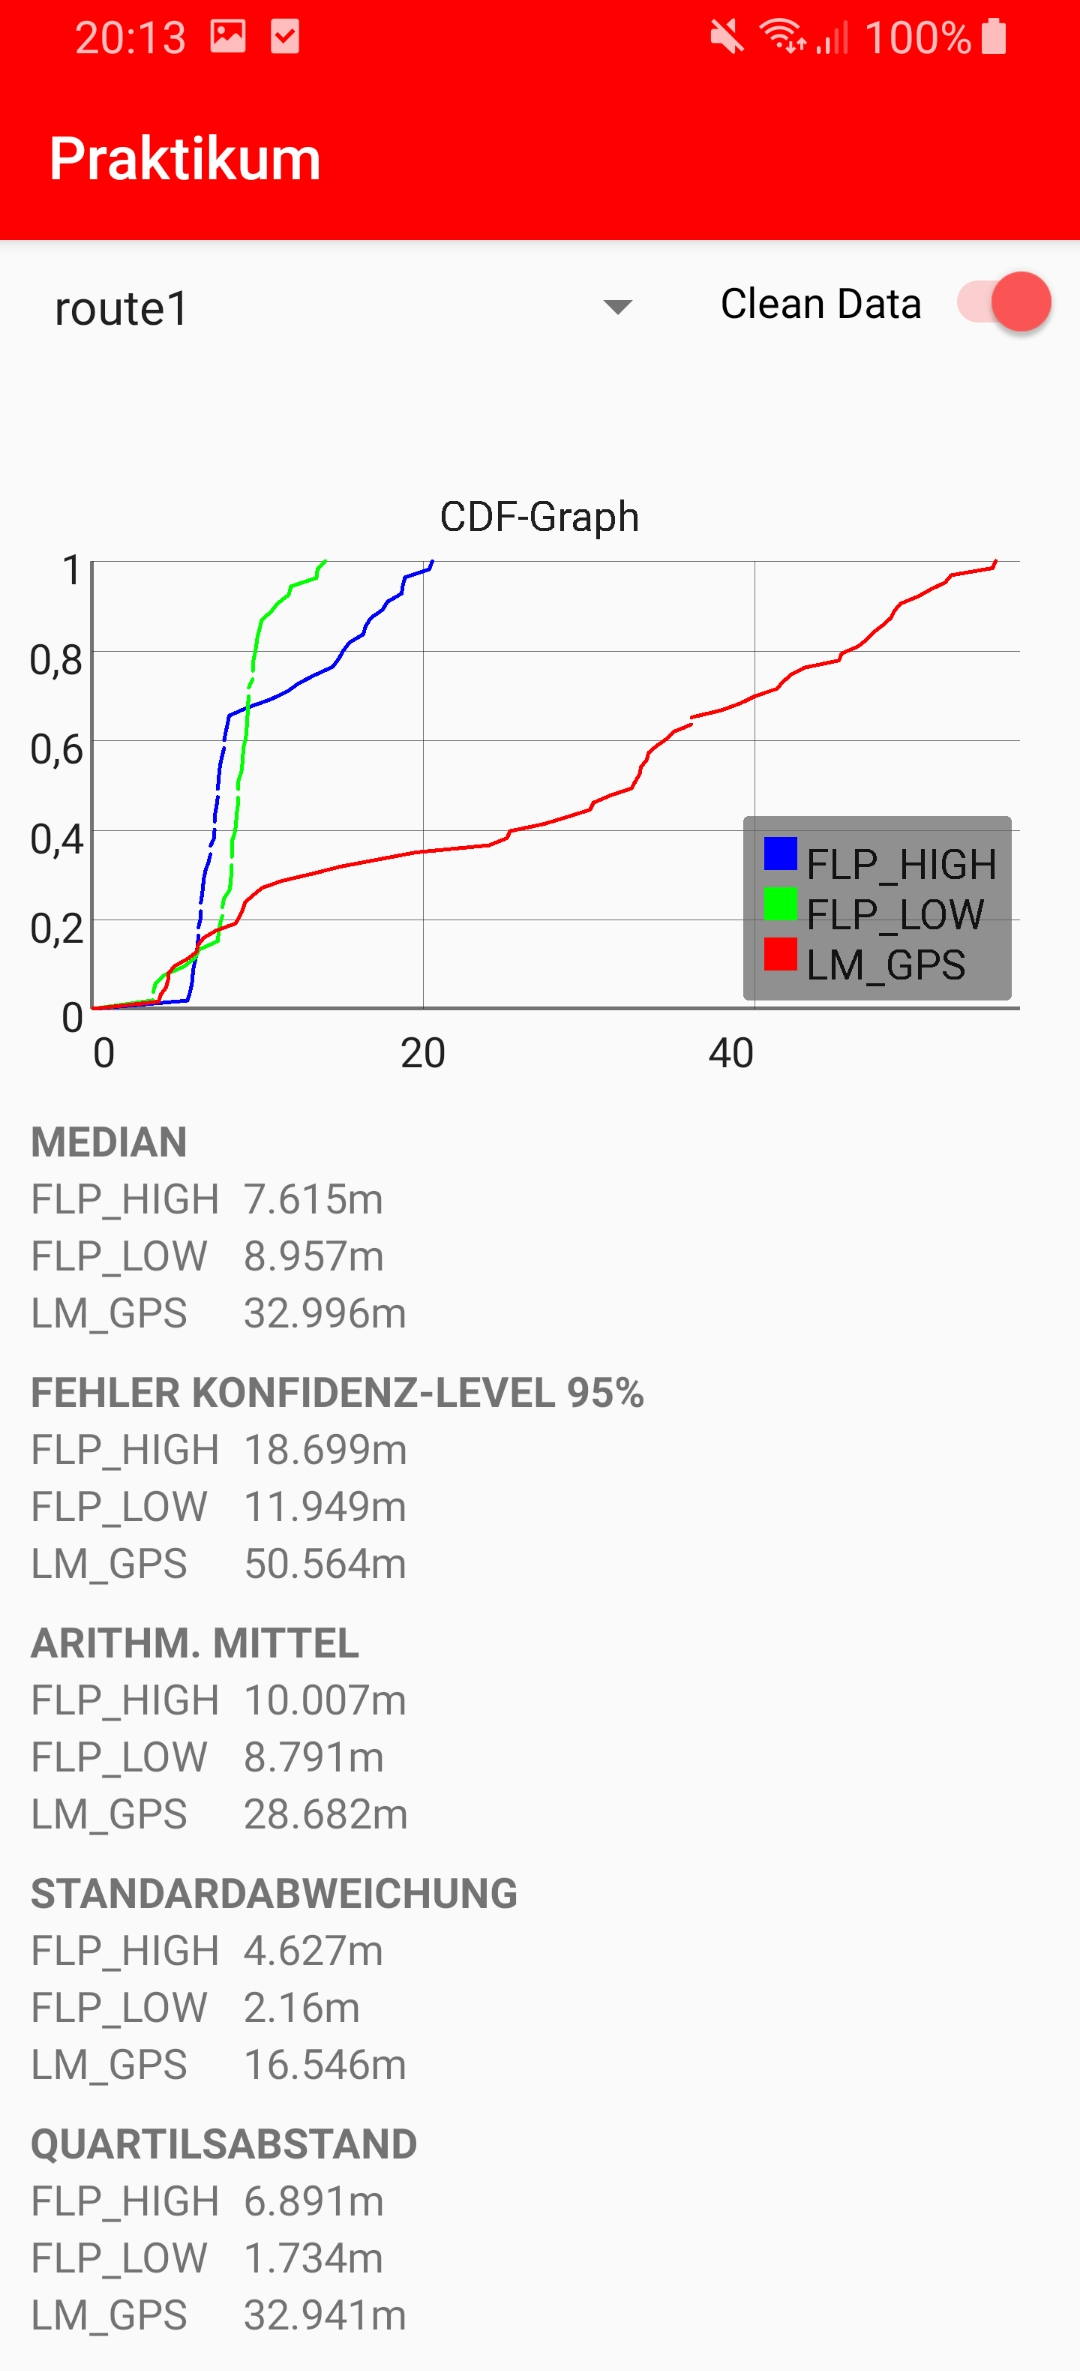
\includegraphics[width=\textwidth]{screenshot_route1}
        \caption{Auswertung Route 1}
        \label{fig:auswertung1}
    \end{subfigure}
    ~ % Abstand
    \begin{subfigure}[b]{0.35\textwidth}
        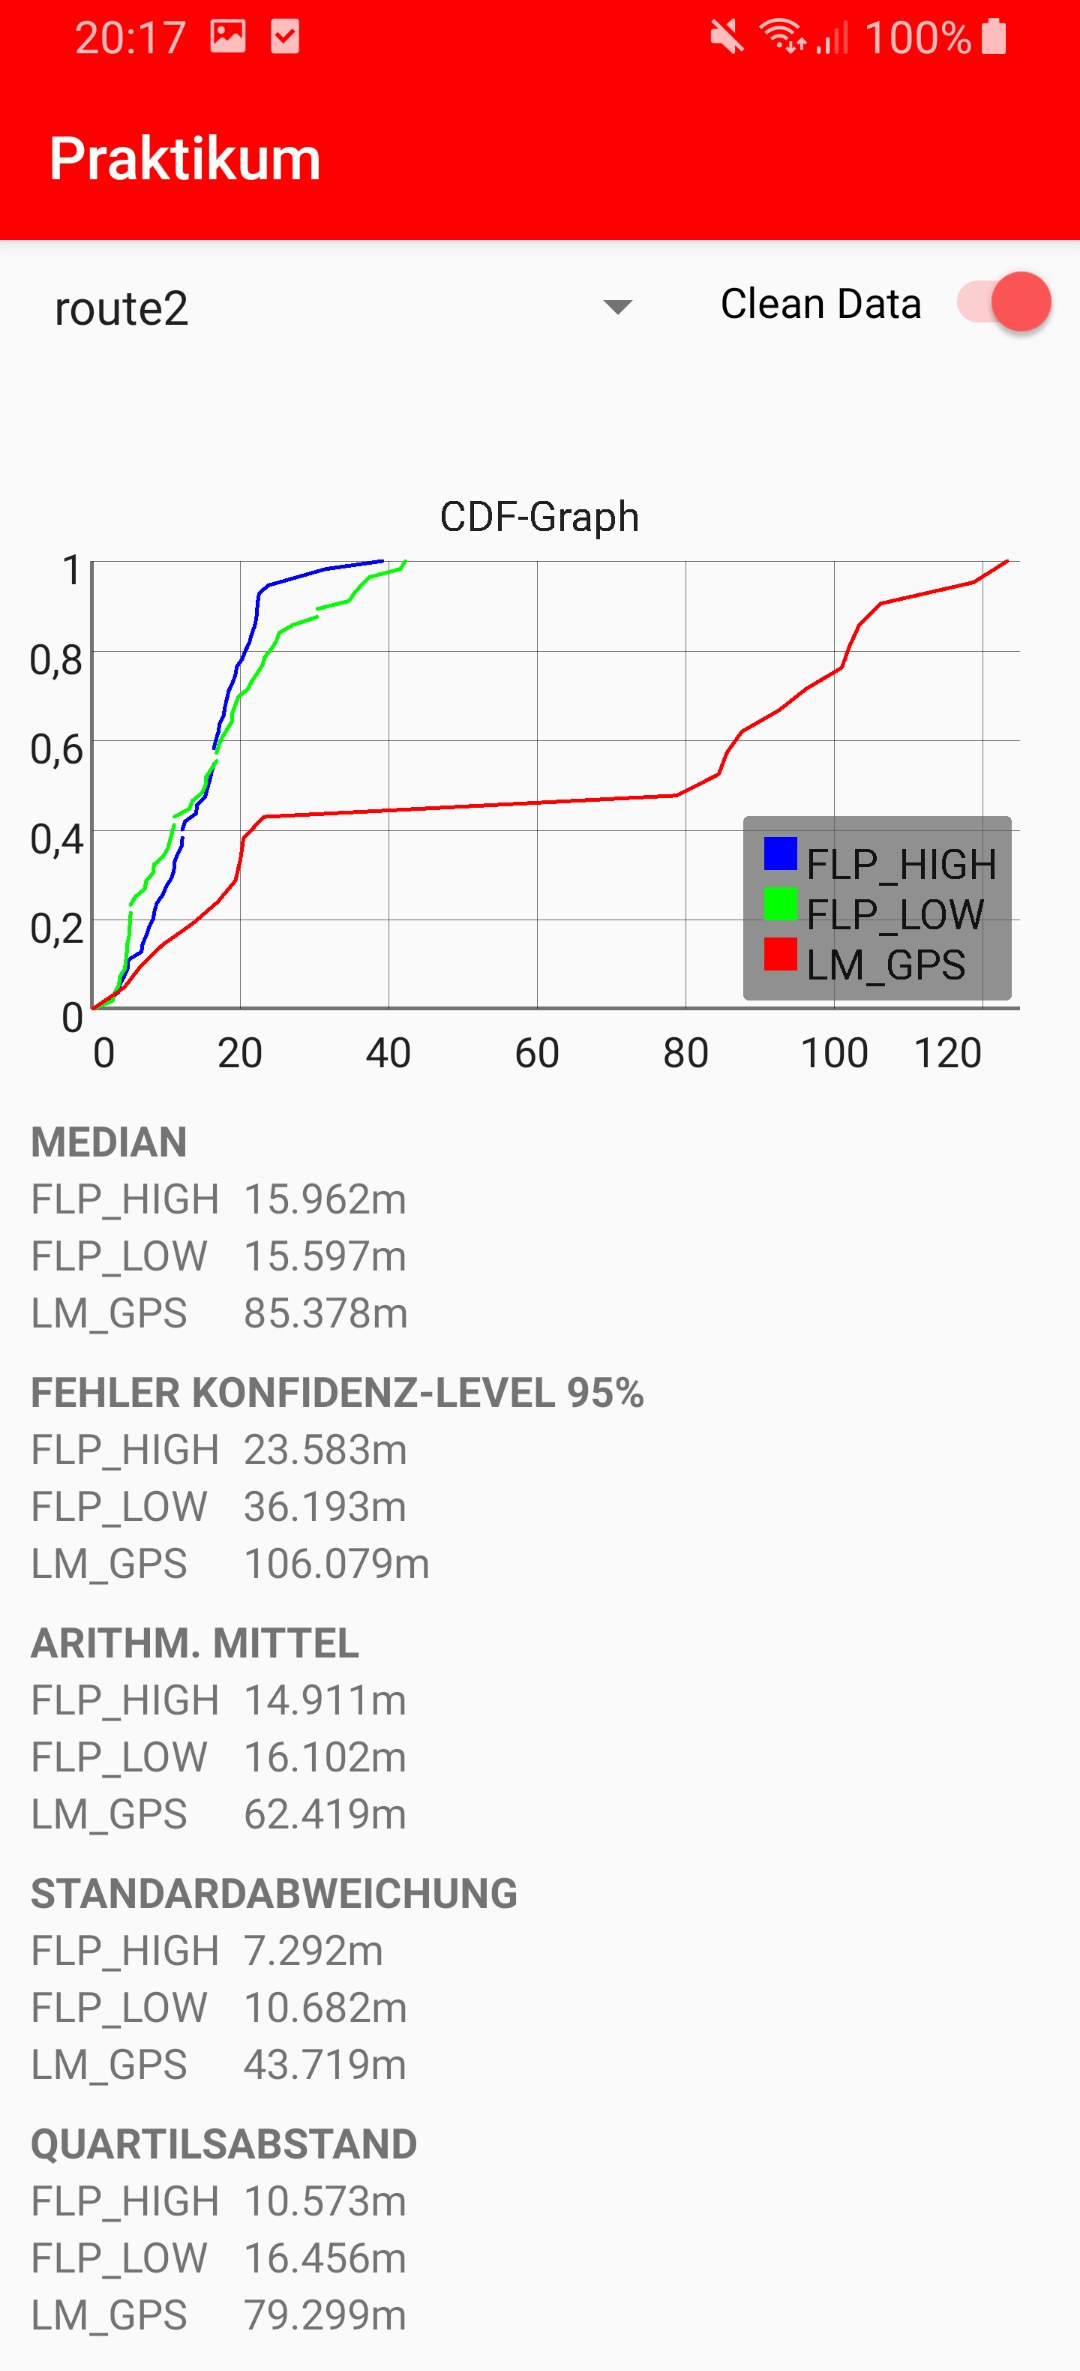
\includegraphics[width=\textwidth]{screenshot_route2}
        \caption{Auswertung Route 2}
        \label{fig:auswertung2}
    \end{subfigure}
    \caption{Auswertung der Routen}
    \label{fig:auswertung}
\end{figure}

\begin{figure}[h!]
    \centering
    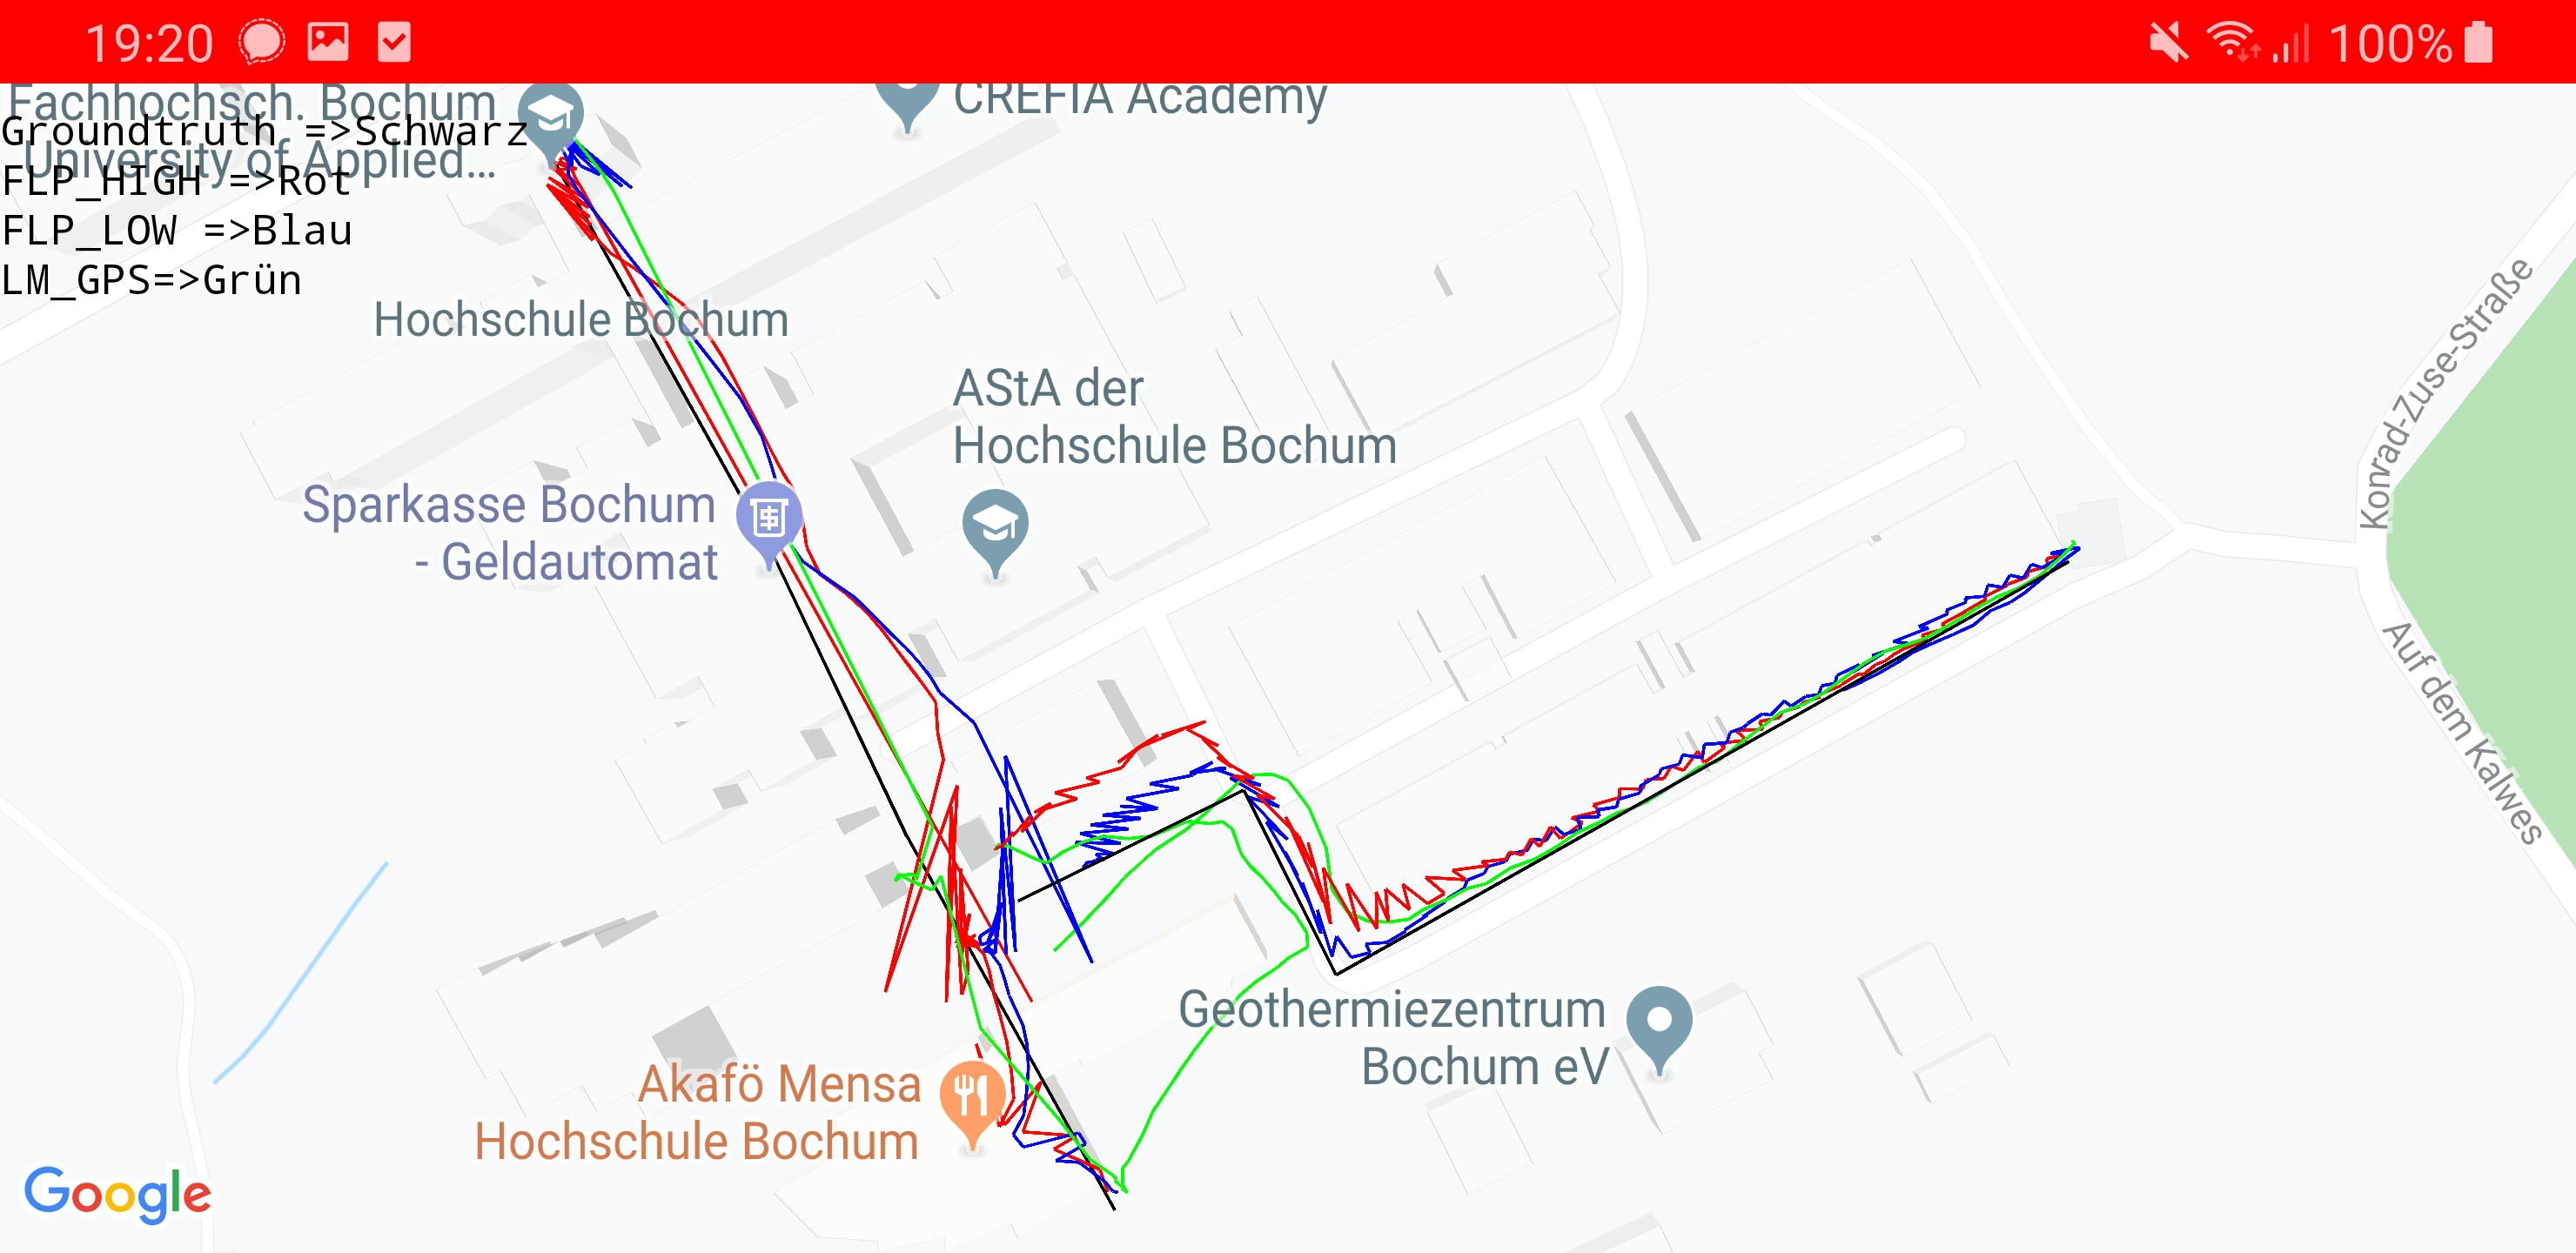
\includegraphics[width=0.8\textwidth]{screenshot_routen_map}
    \caption{Groundtruth und erhobene Daten}
    \label{fig:map}
\end{figure}
	
\end{document}